\chapter{Vector-Vector Inner Product}

This operation takes the equal length of the 
sequence and gives the algebraic sum of the product of the corresponding entries.

Let $x$ and $y$ be the vectors of length $n$, then

$x = 
\begin{bmatrix}
    x_0 \\    
    x_1 \\    
    \vdots \\
    x_n \\    
\end{bmatrix}
,\ y = 
\begin{bmatrix}
    y_0 \\    
    y_1 \\    
    \vdots \\
    y_n \\    
\end{bmatrix}
$

\begin{equation}
    x \cdot y = \sum_{i=0}^{n}(x_i \times y_i)
    \label{equ:dot_prod}
\end{equation}

\begin{equation}
    y \cdot x = x \cdot y
    \label{equ:dot_prod_comm}
\end{equation}

Equation \ref{equ:dot_prod_comm} can be easily proven using equation \ref{equ:dot_prod}.

\[y \cdot x = \sum_{i=0}^{n}(y_i \times x_i)\]

We know that multiplication on a scalar is commutative. Using this fact, we can say
\[y \cdot x = \sum_{i=0}^{n}(x_i \times y_i)\]

From the equation \ref{equ:dot_prod}
\[y \cdot x = x \cdot y\]

\section{Calculating Number of Operations}

Using equation \ref{equ:dot_prod}, we fill the below table

\begin{tabular}{|c|c|}
    \hline
    \textbf{Name} & \textbf{Number} \\
    \hline
    Multiplication & $n$ \\
    \hline
    Addition & $n - 1$ \\
    \hline
\end{tabular}

Total Number of Operations $=$ Number of Multiplication $+$ Number of Addition

Total Number of Operations $= n + (n - 1)$

Total Number of Operations $= 2n - 1$

\section{Algorithm}

\begin{algorithm}[H]
    \SetAlgoLined
    \SetKwFunction{SIMDFn}{simd\_loop}
    \SetKwProg{Fn}{Function}{:}{end}

    \tcp{$a$ is the pointer to the first vector}
    \tcp{$b$ is the pointer to the second vector}
    \tcp{$n$ is the length of the vectors}
    \Fn{\SIMDFn($a$, $b$, $n$)}{
        \assignln{sum}{0}

        \openmp{simd reduction(+:$sum$)}
        \For{\assign{i}{0} \KwTo $n$ \KwBy 1}{
            \assignln{sum}{sum + a[i] \times b[i]}
        }
        \KwRet{$sum$}
    }
    \caption{Inner Product SIMD Function}
\end{algorithm}

\begin{algorithm}[H]
    \SetAlgoLined
    \KwIn{$c$, $a$, $b$, $max\_threads$, $n$}
    \tcp{$a$ and $b$ are pointer to the vectors}
    \tcp{$c$ is the pointer to the output}
    \tcp{$n$ is the size of the vectors}
    \tcp{$max\_threads$ is the user provided thread count}

    \Begin{
        \assignln{number\_el\_L_1}{ \lfloor \frac{S_{L_1}}{S_{data}} \rfloor}
        \assignln{number\_el\_L_2}{\lfloor \frac{S_{L_2}}{S_{data}} \rfloor}
        \assignln{block_1}{2 \times number\_el\_L_1}
        \assignln{block_2}{\lfloor \frac{number\_el\_L_1}{2} \rfloor}
        \assignln{block_3}{\lfloor \frac{number\_el\_L_2}{2} \rfloor}
        \assignln{sum}{0}

        $omp\_set\_num\_threads(max\_threads)$

        \If{$n < block_1$}{
            \assignln{sum}{simd\_loop(a,b,n)}
        }
        \ElseIf{$n < block_3$}{
            \assignln{min\_threads}{\lfloor \frac{n}{block_2} \rfloor}
            \assignln{num\_threads}{max(1, max(min\_threads,max\_threads))}

            $omp\_set\_num\_threads(num\_threads)$

            \openmp{parallel for schedule(static) \textbackslash\ }
            \textbf{reduction(+:$sum$)}\\
            \For{\assign{i}{0} \KwTo n \KwBy $block_2$}{
                \assign{ib}{min( block_2, n - i  )}
                \assign{sum}{sum + simd\_loop(a + i,b + i,ib)}
            }
            
        }
        \Else{
            \openmp{parallel reduction(+:$sum$)}
            \Begin{
                
                \For{\assign{i}{0} \KwTo $ n $ \KwBy $block_3$}{
                    \assignln{ib}{min( block_3,\ n - i )}
                    \assignln{ai}{a + i}
                    \assignln{bi}{b + i}
                    
                    \openmp{for schedule(dynamic)}
                    \For{\assign{j}{0} \KwTo $ ib $ \KwBy $block_2$}{
                        \assignln{jb}{min( block_2,ib - j)}
                        \assign{sum}{sum + simd\_loop(ai + j,bi + j,jb)}
                    }
                }
                
            }
        }
        \assign{c}{sum}
    }

    \caption{Dot Product}
\end{algorithm}

The algorithm fragmented into three sections, and each part represents cache hierarchy.

\subsection{The First Section}

This section handles the data when the vector's length is less than the $S_{L_1}$. 
Here, we do not touch the threads because the overhead incurred is significant 
to paralysis the performance, and we get the worst performance compared with no 
thread or other libraries. When the whole data can fit in the $L_1$ cache, 
it is best not to use threads. We move to the next section when the cache 
misses large enough to compensate for the thread overhead.

According to the \textbf{Amdahl's Law}, we know

\begin{equation}
    Speedup_N = \frac{1}{ p + \frac{1 - p}{N} } - O_N
    \label{equ:amdahls_law}
\end{equation}
$p$ is the proportion of execution time for code that is not parallelizable, where $p \in [0,1]$ \\
$1 - p$ is the proportion of execution time for code that is parallelizable \\
$N$ is the number of processor cores or number of threads, where $N \in Z_{\ne 0}$ \\
$O_N$ is the overhead incurred due to the $N$ thread

Using the equation \ref{equ:amdahls_law}  for $N = 1$, we know the $Speedup_1 = 1$ since 
the program is already running on the thread, and we do not need to spawn another thread. 
Therefore the thread overhead incurred is none ( $O_1 = 0$ ).

In order to perform better than the single-threaded program, 
we need the $Speedup_N$ to exceed the $Speedup_1$ and $N > 1$. 
We can now get the lower bound using the fact and the 
relationship between the vectors' length and the thread overhead.
\[Speedup_N > Speedup_1\]

From the equation \ref{equ:amdahls_law}, we get
\[\frac{1}{ p + \frac{1 - p}{N} } - O_N > 1\]
\begin{align*}
O_N &< \frac{1}{ p + \frac{1 - p}{N} } - 1\\
O_N &< \frac{N}{ Np + 1 - p } - 1\\
O_N &< \frac{N}{ 1 + p(N - 1) } - 1\\
O_N &< \frac{(N - 1) - p(N - 1)}{ 1 + p(N - 1) }\\
O_N &< \frac{(N - 1)(1 - p)}{ 1 + p(N - 1) }\\
O_N &< \frac{1 - p}{ \frac{1}{(N - 1)} + p }
\end{align*}

Let $\frac{1}{N-1}$ be $C_N$ and $C_N \leq 1$, where $N > 1$
\begin{equation}
    O_N < \frac{1 - p}{ C_N + p }
    \label{eq:prop_overhead}
\end{equation}

We know $p \in [0,1]$. Now, we get
\[0 \leq \frac{1 - p}{ C_N + p } \leq \frac{1}{C_N}\]
\[0 \leq O_N < \frac{1}{C_N}\]
\[0 \leq O_N < N - 1\]

Therefore, $O_N \in [0,N-1)$. We can theorise that $p$ must be a function of Block ($B_1$).
\begin{align*}
    p &\propto B_1\\
    p &= kB_1
\end{align*}
where $k$ is the proportionality constant. Now, replace $p$ in the equation \ref{eq:prop_overhead}
\begin{align*}
    O_N &< \frac{1}{ \frac{C_N + kB_1}{1 - kB_1} }\\
\end{align*}

As we $B_1$ increase then $1 - kB_1$ decrease and $C_N + kB_1$ also increase, which over all decrease
the overhead ($O_N$)

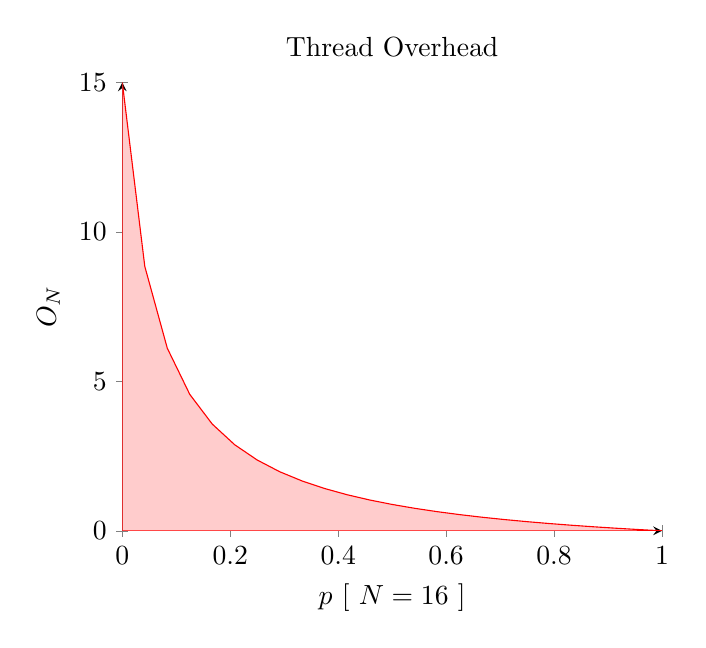
\begin{tikzpicture}
    \begin{axis}[
        title = {Thread Overhead},
        axis lines = left,
        xlabel={$p$ [ $N = 16$ ]},
        ylabel=$O_N$,
    ]

    \addplot[
        domain=0:1,
        color=red,
        fill=red!20,
    ]{((1-x)/((1 / 15) + x))} \closedcycle;
    
    \end{axis}
\end{tikzpicture}

The $B_1$'s lower bound found to be the number of elements that can be fit inside 
the $L_1$ cache through the experimental data. This phenomenon happens because 
the vectors' elements cannot fit inside the cache, and cache misses increase, 
dominating the thread overhead.

\[B_1 \geq \frac{S_{L_1}}{S_{data}}\]

However, the optimal block size for this section found to be twice 
the vectors' elements that can put inside the cache.

\begin{equation}
    B_1 = \frac{2S_{L_1}}{S_{data}}
    \label{eq:dot_block1}
\end{equation}

\textbf{Experimental Data for $B_1$}

\begin{figure}[htb]
    \centering
    \subfloat[\centering Single-Precision]{{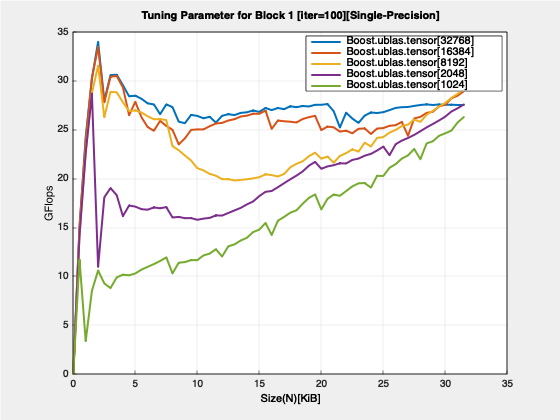
\includegraphics[width=5cm]{../assets/dot_product/tuning_block_one_float.png} }}%
    \label{fig:dot_Stuning_block1}
    \qquad
    \subfloat[\centering Double-Precision]{{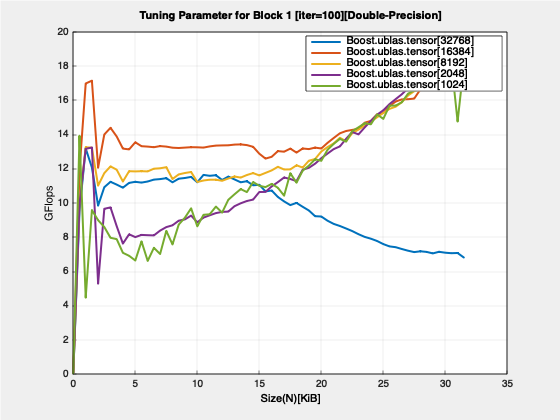
\includegraphics[width=5cm]{../assets/dot_product/tuning_block_one_double.png} }}%
    \label{fig:dot_Dtuning_block1}
\end{figure}

\begin{tabular}{l|c|c|}
    & \textbf{Block[Single]} & \textbf{Block[Double]}\\
    \hline
    \textbf{Lower Bound} & 8192 (8K) & 4096 (4K)\\
    \hline
    \textbf{Optimal} & 16384 (16K) & 8192 (8K)\\
    \hline
\end{tabular}

\subsection{The Second Section}

Here, the cache misses is large enough to dominate the thread overhead, 
and the thread can provide speedup more significant than a single thread. 
To quench the data demand for each thread, we fit both vectors' elements 
inside the $L_1$ cache, and the accumulator always is inside the register—the 
whole $L_1$ cache used for vectors. The advantage of the threads come in handy 
because most of the CPU architecture provides a private $L_1$ cache, which 
owned by each core, and as the inner product is an independent operation, 
no two elements are dependent on each other for the result. 
Each private $L_1$ cache can fetch a different part of the sequence 
and run in parallel without waiting for the result to come from another thread, 
because of which there is no need to invalidate the cache. Once the data comes 
inside the $L_1$ cache, it will compute a fragment of the sequence and keeps 
the accumulated result in the register and then fetch another part. 
In the end, it will combine all the partial results into one final result.

\[S_{L_1} = S_{data}(Block\ of\ the\ first\ vector + Block\ of\ the\ second\ vector)\]

From the equation \ref{equ:dot_prod}, we can infer that the block of both vectors must
be equal to give the optimal block size.

\[B_2 = Block\ of\ the\ first\ vector = Block\ of\ the\ second\ vector\]

\begin{align*}
    S_{L_1} &= S_{data}(B_2 + B_2)\\
    S_{L_1} &= 2S_{data}B_2\\
\end{align*}

\begin{equation}
    B_2 = \frac{S_{L_1}}{2S_{data}}
    \label{eq:dot_block2}
\end{equation}

\newpage
\textbf{Experimental Data for $B_2$}

\begin{figure}[htb]
    \centering
    \subfloat[\centering Single-Precision]{{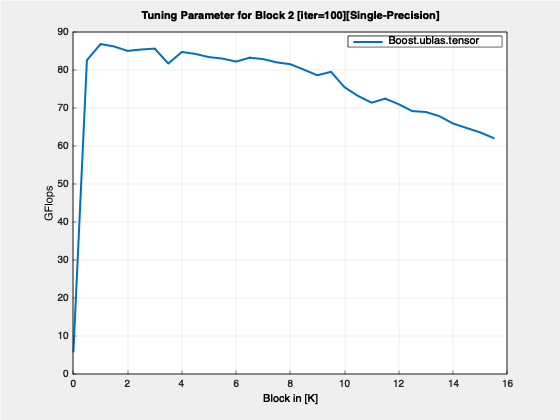
\includegraphics[width=5cm]{../assets/dot_product/tuning_block_two_float.png} }}%
    \label{fig:dot_Stuning_block2}
    \qquad
    \subfloat[\centering Double-Precision]{{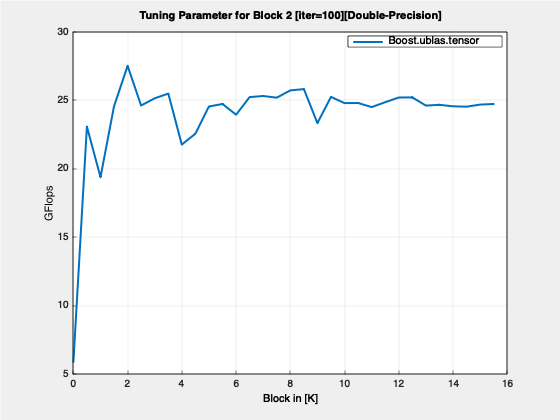
\includegraphics[width=5cm]{../assets/dot_product/tuning_block_two_double.png} }}%
    \label{fig:dot_Dtuning_block2}
\end{figure}

\begin{tabular}{l|c|c|}
    & \textbf{Block[Single]} & \textbf{Block[Double]}\\
    \hline
    \textbf{Theoretical Optimal} & 4096 (4K) & 2048 (2K)\\
    \hline
    \textbf{Experimental Optimal} & 4096 (4K) & 2048 (2K)\\
    \hline
\end{tabular}

\subsection{The Third Section}

Here, once the data starts to exceed the $L_2$ cache or even $L_3$ cache, 
we use the CPU architecture's prefetch feature. 
This section may or may not affect some architecture; 
if the $L_2$ cache is also private for different cores, 
it will prefetch the data and fill it, and when it goes 
inside the loop, which utilizes the threads will fetch 
the data into the L1 cache from the $L_2$ cache. 
If the $L_2$ shared among all the cores, the gain might be 
minimal or see no gain in speedup. With the same logic 
we used to derive equation \ref{eq:dot_block2}, we can use it here also.

\[S_{L_2} = S_{data}(Block\ of\ the\ first\ vector + Block\ of\ the\ second\ vector)\]

From the equation \ref{equ:dot_prod}, we can infer that the block of both vectors must
be equal to give the optimal block size.

\[B_3 = Block\ of\ the\ first\ vector = Block\ of\ the\ second\ vector\]

\begin{align*}
    S_{L_2} &= S_{data}(B_3 + B_3)\\
    S_{L_2} &= 2S_{data}B_3\\
\end{align*}

\begin{equation}
    B_3 = \frac{S_{L_2}}{2S_{data}}
    \label{eq:dot_block3}
\end{equation}

\newpage
\textbf{Experimental Data for $B_2$}

\begin{figure}[htb]
    \centering
    \subfloat[\centering Single-Precision]{{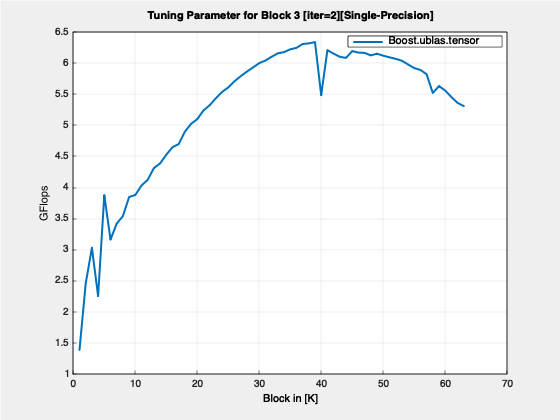
\includegraphics[width=5cm]{../assets/dot_product/tuning_block_three_float.png} }}%
    \label{fig:dot_Stuning_block3}
    \qquad
    \subfloat[\centering Double-Precision]{{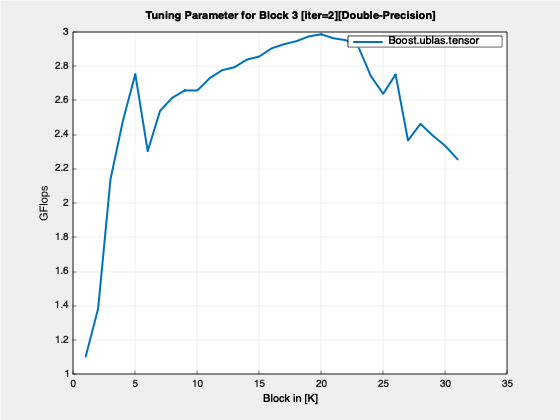
\includegraphics[width=5cm]{../assets/dot_product/tuning_block_three_double.png} }}%
    \label{fig:dot_Dtuning_block3}
\end{figure}

\begin{tabular}{l|c|c|}
    & \textbf{Block[Single]} & \textbf{Block[Double]}\\
    \hline
    \textbf{Theoretical Optimal} & 32768 (32K) & 16384 (16K)\\
    \hline
    \textbf{Experimental Optimal} & $\geq$ 30K and $\leq$ 40K & $\geq$ 16K and $\leq$ 20K\\
    \hline
\end{tabular}

\section{Performance Plots and Speedup Summary}

\subsection{Range[Start: $2$, End: $2^{20}$, Step: $1024$]}

\subsubsection{Performance measurements of ?dot implementations}
\begin{figure}[htb]
    \centering
    \subfloat[\centering Single-Precision]{{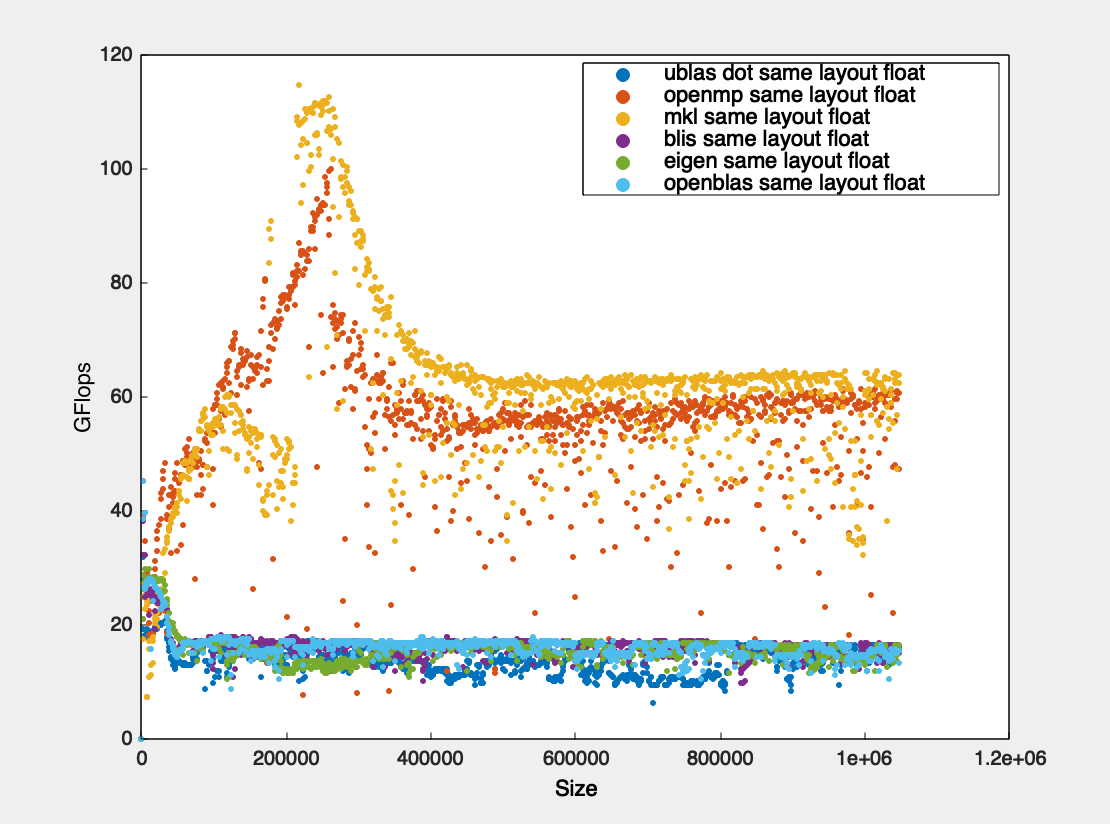
\includegraphics[width=5cm]{../assets/dot_product/plot_2^20/float_GflopsVsSize.png} }}%
    \label{fig:dot_Sgflop220}
    \qquad
    \subfloat[\centering Double-Precision]{{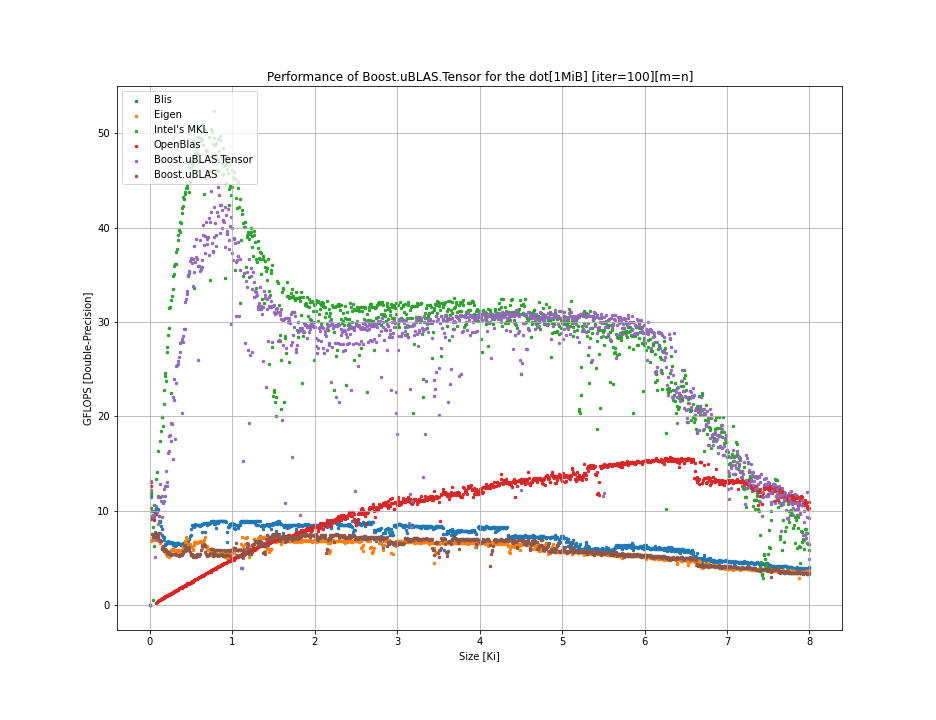
\includegraphics[width=5cm]{../assets/dot_product/plot_2^20/double_GflopsVsSize.png} }}%
    \label{fig:dot_Dgflop220}
\end{figure}

\newpage
\subsubsection{Sorted performance measurements of ?dot implementations}
\begin{figure}[htb]
    \centering
    \subfloat[\centering Single-Precision]{{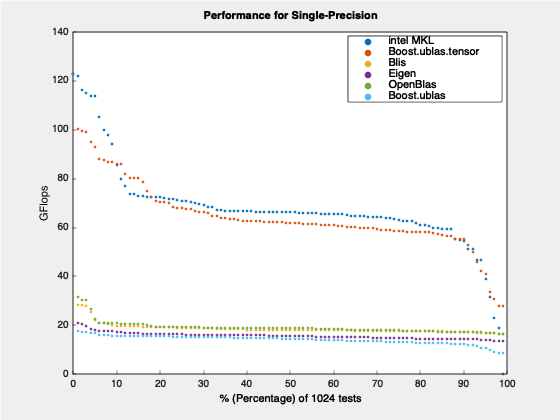
\includegraphics[width=5cm]{../assets/dot_product/plot_2^20/float_GflopsVsSize_per.png} }}%
    \label{fig:dot_Sgflop_per220}
    \qquad
    \subfloat[\centering Double-Precision]{{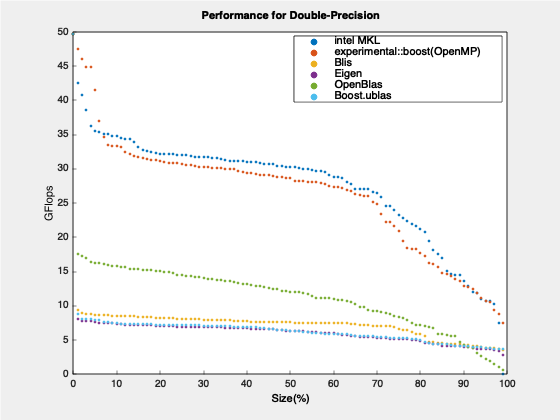
\includegraphics[width=5cm]{../assets/dot_product/plot_2^20/double_GflopsVsSize_per.png} }}%
    \label{fig:dot_Dgflop_per220}
\end{figure}

\subsubsection{Comparison of the Boost.uBLAS.Tensor ?dot implementation}
\begin{figure}[htb]
    \centering
    \subfloat[\centering Single-Precision]{{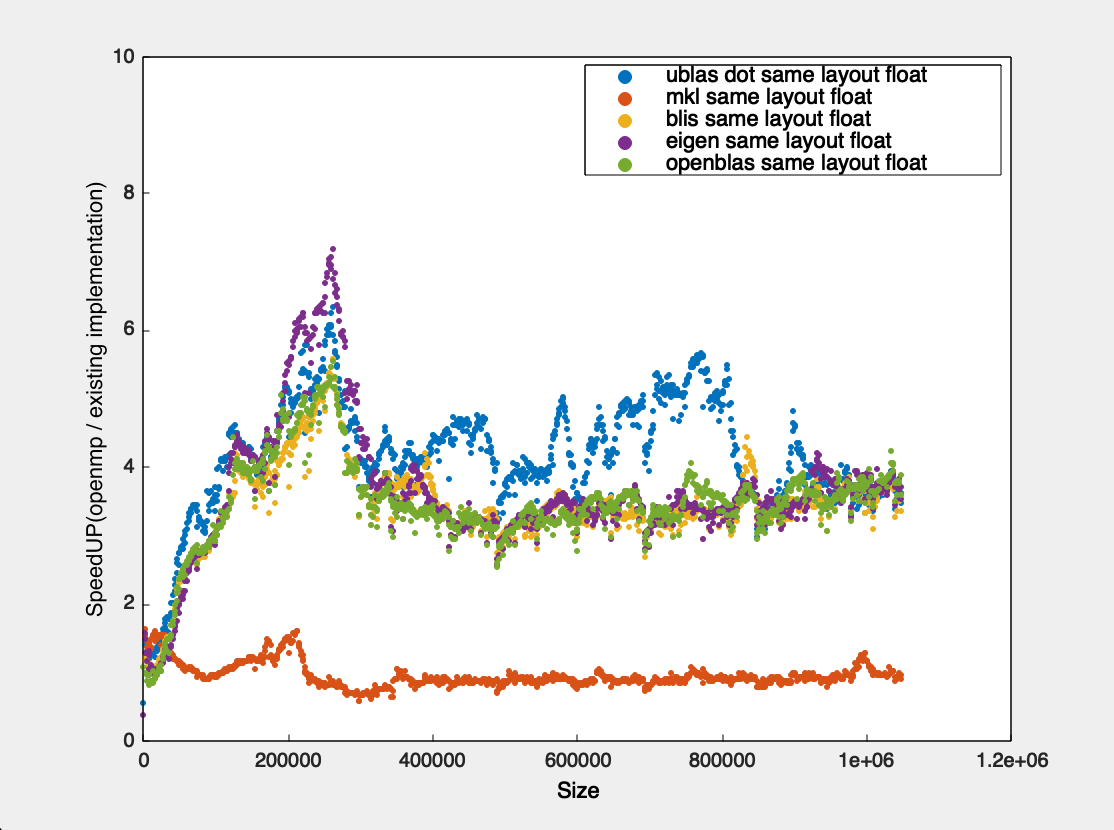
\includegraphics[width=5cm]{../assets/dot_product/plot_2^20/float_Speedup(openmp).png} }}%
    \label{fig:dot_Sspeedup220}
    \qquad
    \subfloat[\centering Double-Precision]{{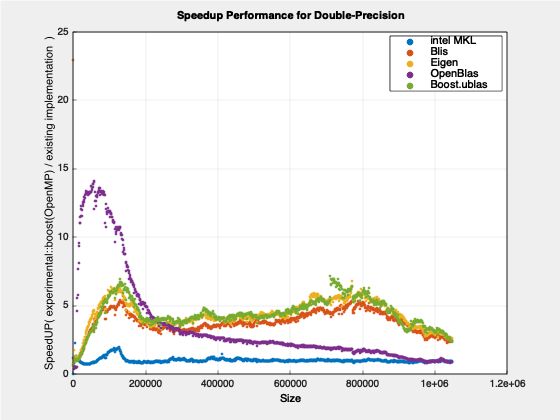
\includegraphics[width=5cm]{../assets/dot_product/plot_2^20/double_Speedup(openmp).png} }}%
    \label{fig:dot_Dspeedup220}
\end{figure}

\subsubsection{Comparison of the Boost.uBLAS.Tensor ?dot implementation [semilogy]}
\begin{figure}[htb]
    \centering
    \subfloat[\centering Single-Precision]{{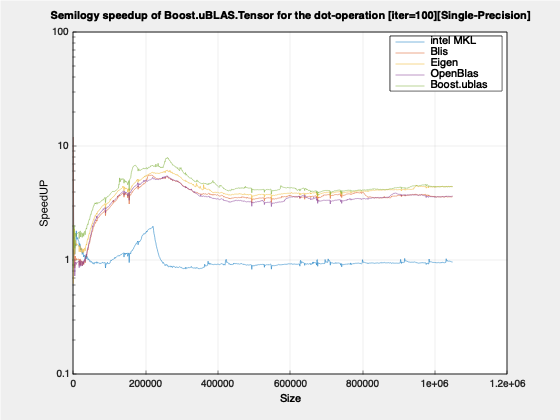
\includegraphics[width=5cm]{../assets/dot_product/plot_2^20/float_Speedup_log10(openmp).png} }}%
    \label{fig:dot_Sspeedup_log10220}
    \qquad
    \subfloat[\centering Double-Precision]{{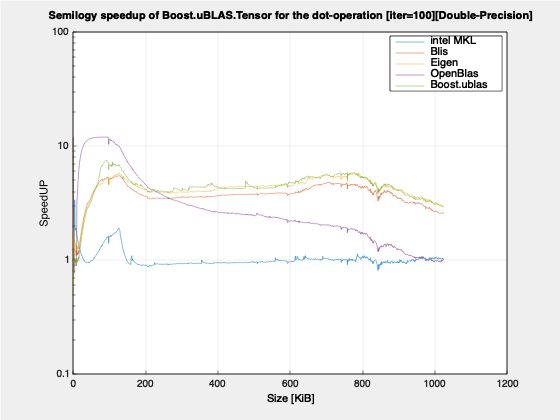
\includegraphics[width=5cm]{../assets/dot_product/plot_2^20/double_Speedup_log10(openmp).png} }}%
    \label{fig:dot_Dspeedup_log10220}
\end{figure}

\newpage
\subsubsection{Comparison of the Boost.uBLAS.Tensor ?dot implementation [sorted]}
\begin{figure}[htb]
    \centering
    \subfloat[\centering Single-Precision]{{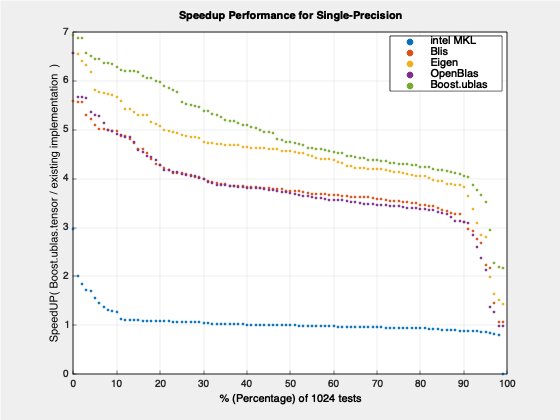
\includegraphics[width=5cm]{../assets/dot_product/plot_2^20/float_Speedup_per(openmp).png} }}%
    \label{fig:dot_Sspeedup_per220}
    \qquad
    \subfloat[\centering Double-Precision]{{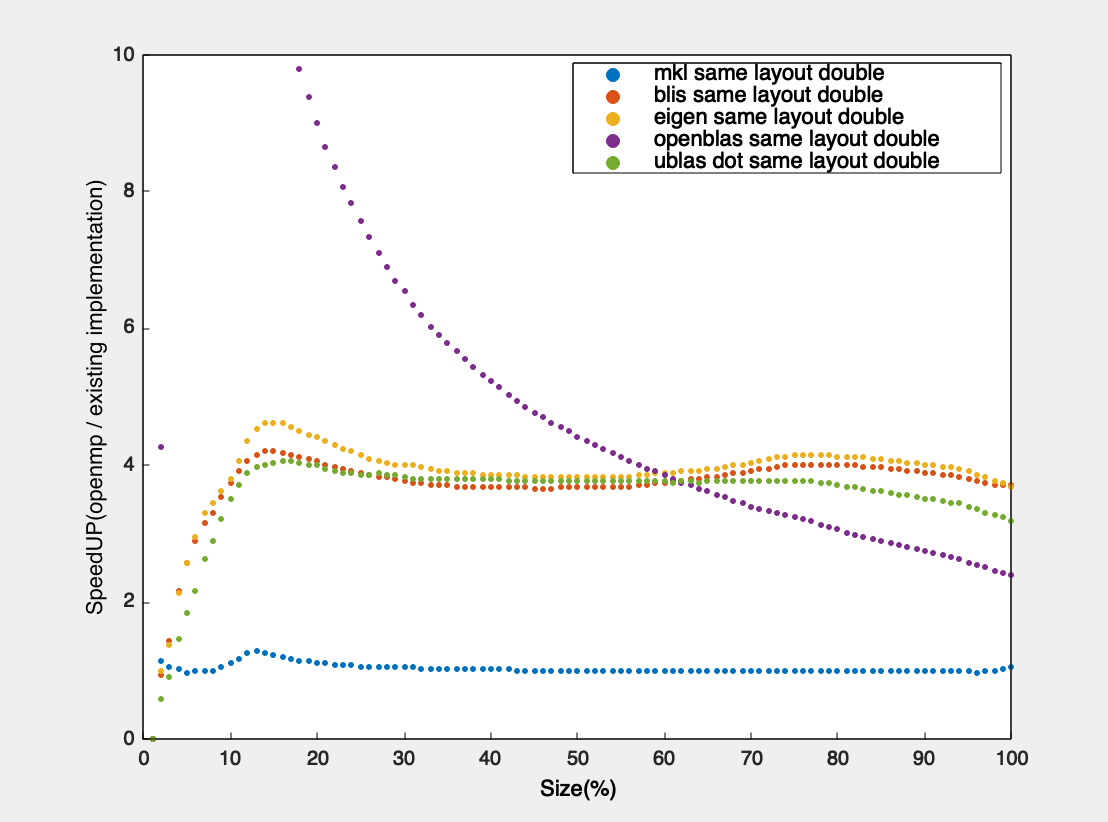
\includegraphics[width=5cm]{../assets/dot_product/plot_2^20/double_Speedup_per(openmp).png} }}%
    \label{fig:dot_Dspeedup_per220}
\end{figure}

\begin{table}[ht]
    \centering
    \caption{Speedup Summary For Single-Precision}
    \begin{tabular}{|l|c|c|}
        \hline
        \textbf{Implementation} & \textbf{Speedup $\geq$ 1 [\%]} & \textbf{Speedup $\geq$ 2 [\%]}\\
        \hline
        Boost.uBLAS & $99$ & $96$ \\
        \hline
        OpenBLAS    & $98$ & $95$ \\
        \hline
        Eigen       & $99$ & $96$ \\
        \hline
        Blis        & $98$ & $96$ \\
        \hline
        Intel's MKL & $62$ & $0$ \\
        \hline
    \end{tabular}
    \newline
    \vspace*{1 cm}
    \newline
    \begin{tabular}{|l|c|c|}
        \hline
        \textbf{Implementation} & \textbf{Speed-down $\geq$ 1 [\%]} & \textbf{Speed-down $\geq$ 2 [\%]}\\
        \hline
        Boost.uBLAS & $0$ & $0$ \\
        \hline
        OpenBLAS    & $0$ & $0$ \\
        \hline
        Eigen       & $0$ & $0$ \\
        \hline
        Blis        & $0$ & $0$ \\
        \hline
        Intel's MKL & $35$ & $0$ \\
        \hline
    \end{tabular}
\end{table}

\begin{table}[ht]
    \centering
    \caption{Speedup Summary For Double-Precision}
    \begin{tabular}{|l|c|c|}
        \hline
        \textbf{Implementation} & \textbf{Speedup $\geq$ 1 [\%]} & \textbf{Speedup $\geq$ 2 [\%]}\\
        \hline
        Boost.uBLAS & $99$ & $97$ \\
        \hline
        OpenBLAS    & $99$ & $75$ \\
        \hline
        Eigen       & $99$ & $97$ \\
        \hline
        Blis        & $99$ & $98$ \\
        \hline
        Intel's MKL & $88$ & $1$ \\
        \hline
    \end{tabular}
    \newline
    \vspace*{1 cm}
    \newline
    \begin{tabular}{|l|c|c|}
        \hline
        \textbf{Implementation} & \textbf{Speed-down $\geq$ 1 [\%]} & \textbf{Speed-down $\geq$ 2 [\%]}\\
        \hline
        Boost.uBLAS & $0$ & $0$ \\
        \hline
        OpenBLAS    & $0$ & $0$ \\
        \hline
        Eigen       & $0$ & $0$ \\
        \hline
        Blis        & $0$ & $0$ \\
        \hline
        Intel's MKL & $9$ & $0$ \\
        \hline
    \end{tabular}
\end{table}

\newpage
\subsection{Range[Start: $32$, End: $16382$, Step: $32$]}

\subsubsection{Performance measurements of ?dot implementations}
\begin{figure}[htb]
    \centering
    \subfloat[\centering Single-Precision]{{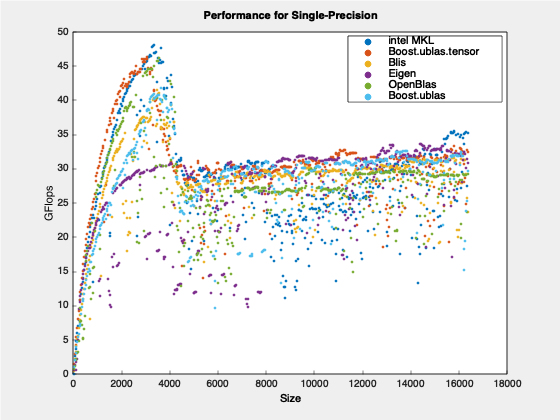
\includegraphics[width=5cm]{../assets/dot_product/plot_ 16382/float_GflopsVsSize.png} }}%
    \label{fig:dot_Sgflop16382}
    \qquad
    \subfloat[\centering Double-Precision]{{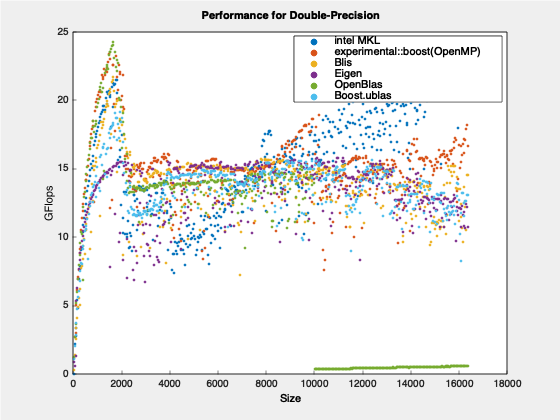
\includegraphics[width=5cm]{../assets/dot_product/plot_ 16382/double_GflopsVsSize.png} }}%
    \label{fig:dot_Dgflop16382}
\end{figure}

\newpage
\subsubsection{Sorted performance measurements of ?dot implementations}
\begin{figure}[htb]
    \centering
    \subfloat[\centering Single-Precision]{{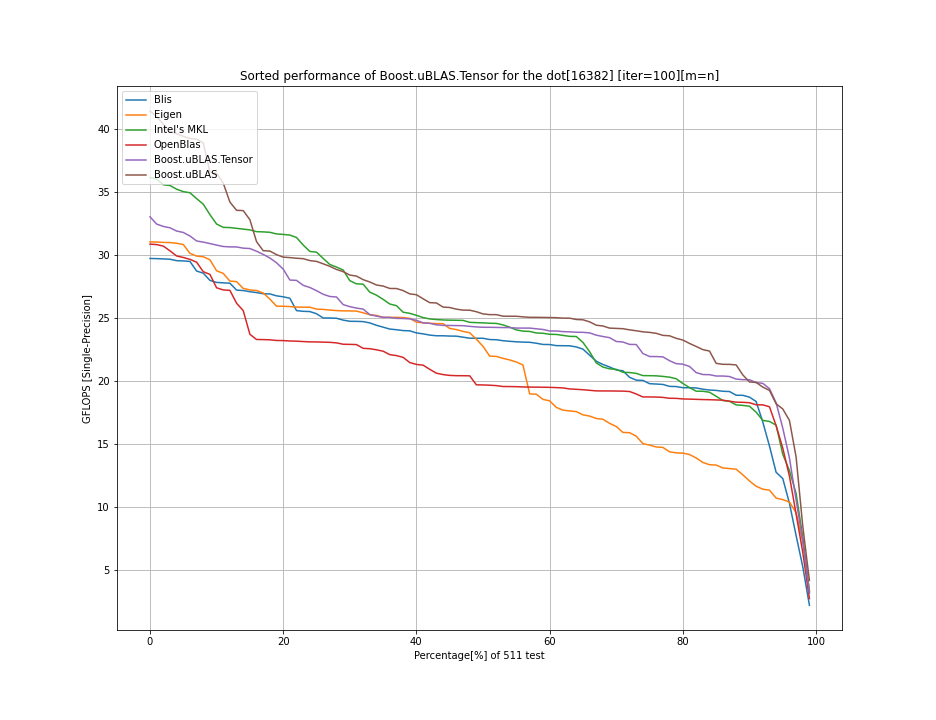
\includegraphics[width=5cm]{../assets/dot_product/plot_ 16382/float_GflopsVsSize_per.png} }}%
    \label{fig:dot_Sgflop_per16382}
    \qquad
    \subfloat[\centering Double-Precision]{{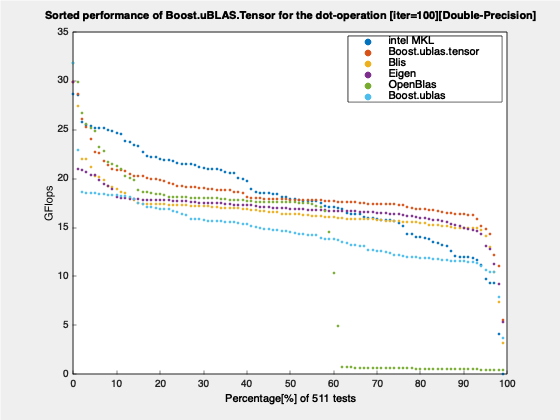
\includegraphics[width=5cm]{../assets/dot_product/plot_ 16382/double_GflopsVsSize_per.png} }}%
    \label{fig:dot_Dgflop_per16382}
\end{figure}

\subsubsection{Comparison of the Boost.uBLAS.Tensor ?dot implementation}
\begin{figure}[htb]
    \centering
    \subfloat[\centering Single-Precision]{{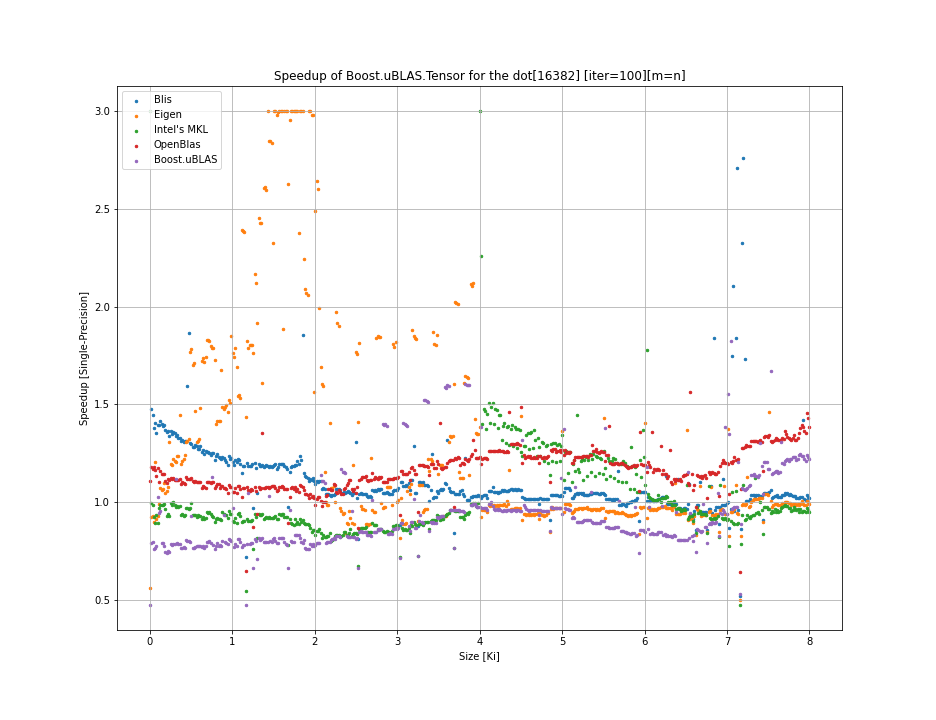
\includegraphics[width=5cm]{../assets/dot_product/plot_ 16382/float_Speedup(openmp).png} }}%
    \label{fig:dot_Sspeedup16382}
    \qquad
    \subfloat[\centering Double-Precision]{{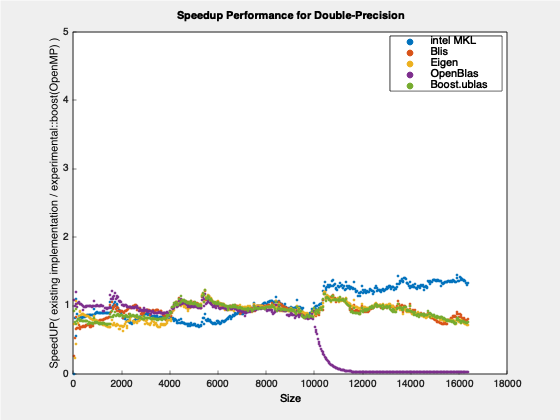
\includegraphics[width=5cm]{../assets/dot_product/plot_ 16382/double_Speedup(openmp).png} }}%
    \label{fig:dot_Dspeedup16382}
\end{figure}

\subsubsection{Comparison of the Boost.uBLAS.Tensor ?dot implementation [semilogy]}
\begin{figure}[htb]
    \centering
    \subfloat[\centering Single-Precision]{{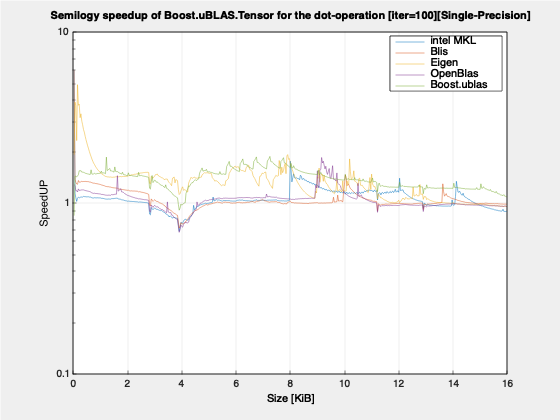
\includegraphics[width=5cm]{../assets/dot_product/plot_ 16382/float_Speedup_log10(openmp).png} }}%
    \label{fig:dot_Sspeedup_log1016382}
    \qquad
    \subfloat[\centering Double-Precision]{{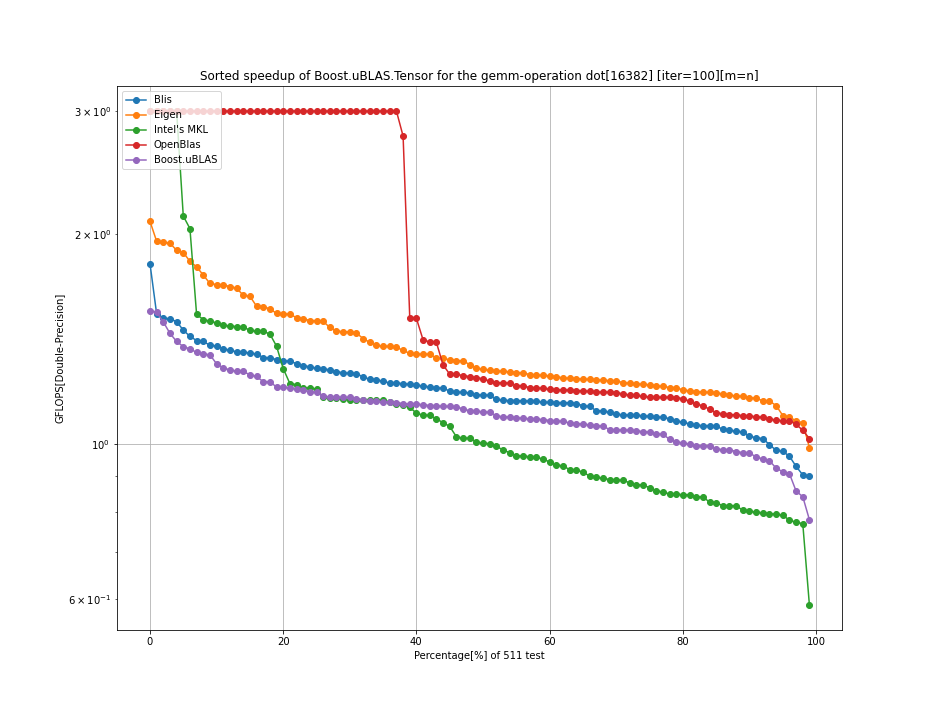
\includegraphics[width=5cm]{../assets/dot_product/plot_ 16382/double_Speedup_log10(openmp).png} }}%
    \label{fig:dot_Dspeedup_log1016382}
\end{figure}

\newpage
\subsubsection{Comparison of the Boost.uBLAS.Tensor ?dot implementation [sorted]}
\begin{figure}[htb]
    \centering
    \subfloat[\centering Single-Precision]{{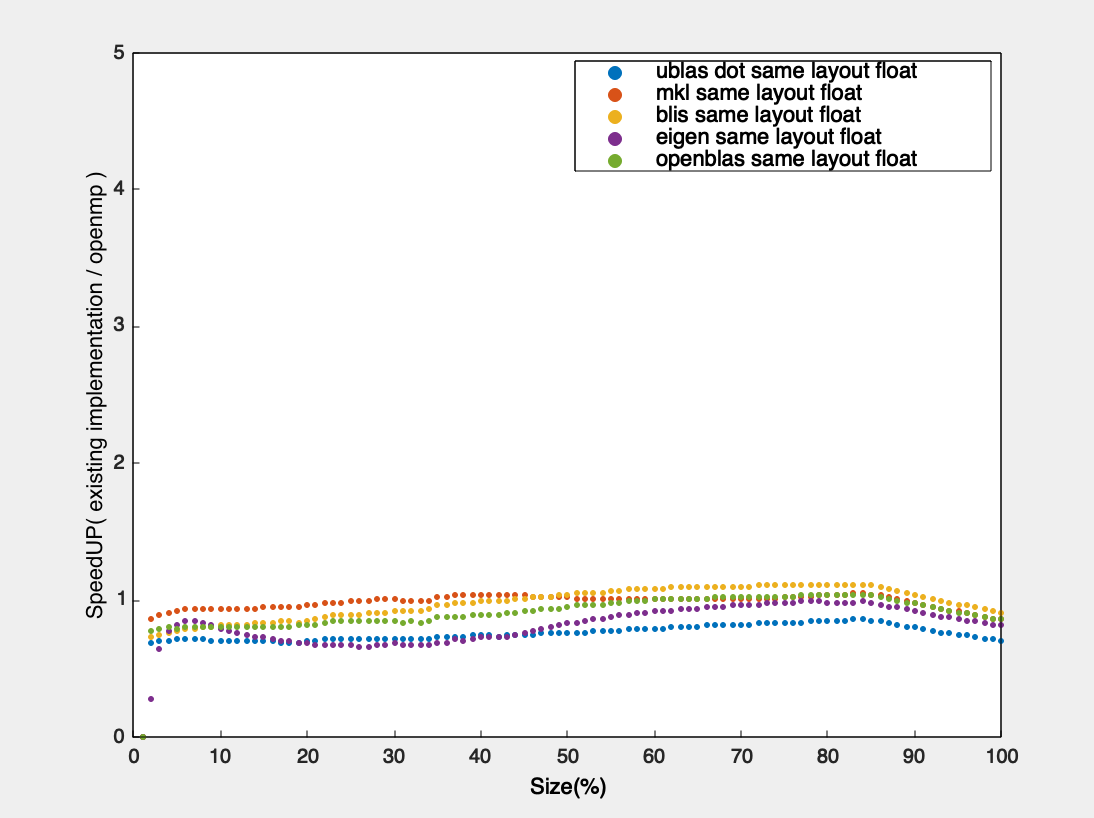
\includegraphics[width=5cm]{../assets/dot_product/plot_ 16382/float_Speedup_per(openmp).png} }}%
    \label{fig:dot_Sspeedup_per16382}
    \qquad
    \subfloat[\centering Double-Precision]{{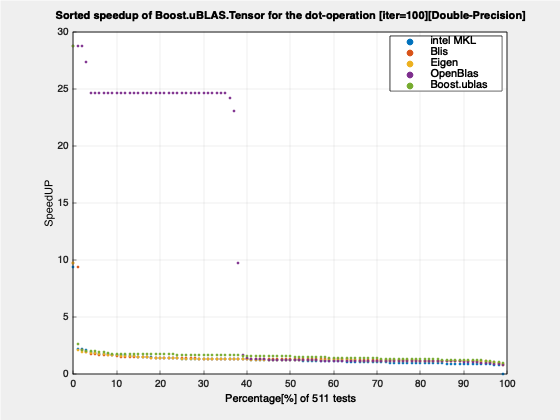
\includegraphics[width=5cm]{../assets/dot_product/plot_ 16382/double_Speedup_per(openmp).png} }}%
    \label{fig:dot_Dspeedup_per16382}
\end{figure}

\begin{table}[ht]
    \centering
    \caption{Speedup Summary For Single-Precision}
    \begin{tabular}{|l|c|c|}
        \hline
        \textbf{Implementation} & \textbf{Speedup $\geq$ 1 [\%]} & \textbf{Speedup $\geq$ 2 [\%]}\\
        \hline
        Boost.uBLAS & $99$ & $7$ \\
        \hline
        OpenBLAS    & $97$ & $6$ \\
        \hline
        Eigen       & $99$ & $13$ \\
        \hline
        Blis        & $98$ & $1$ \\
        \hline
        Intel's MKL & $94$ & $5$ \\
        \hline
    \end{tabular}
    \newline
    \vspace*{1 cm}
    \newline
    \begin{tabular}{|l|c|c|}
        \hline
        \textbf{Implementation} & \textbf{Speed-down $\geq$ 1 [\%]} & \textbf{Speed-down $\geq$ 2 [\%]}\\
        \hline
        Boost.uBLAS & $0$ & $0$ \\
        \hline
        OpenBLAS    & $1$ & $0$ \\
        \hline
        Eigen       & $0$ & $0$ \\
        \hline
        Blis        & $0$ & $0$ \\
        \hline
        Intel's MKL & $3$ & $0$ \\
        \hline
    \end{tabular}
\end{table}

\begin{table}[ht]
    \centering
    \caption{Speedup Summary For Double-Precision}
    \begin{tabular}{|l|c|c|}
        \hline
        \textbf{Implementation} & \textbf{Speedup $\geq$ 1 [\%]} & \textbf{Speedup $\geq$ 2 [\%]}\\
        \hline
        Boost.uBLAS & $99$ & $97$ \\
        \hline
        OpenBLAS    & $99$ & $38$ \\
        \hline
        Eigen       & $99$ & $6$ \\
        \hline
        Blis        & $99$ & $3$ \\
        \hline
        Intel's MKL & $71$ & $2$ \\
        \hline
    \end{tabular}
    \newline
    \vspace*{1 cm}
    \newline
    \begin{tabular}{|l|c|c|}
        \hline
        \textbf{Implementation} & \textbf{Speed-down $\geq$ 1 [\%]} & \textbf{Speed-down $\geq$ 2 [\%]}\\
        \hline
        Boost.uBLAS & $0$ & $0$ \\
        \hline
        OpenBLAS    & $3$ & $0$ \\
        \hline
        Eigen       & $0$ & $0$ \\
        \hline
        Blis        & $0$ & $0$ \\
        \hline
        Intel's MKL & $26$ & $0$ \\
        \hline
    \end{tabular}
\end{table}

\newpage
\section{Performance Metrics}

\subsection*{Range[Start: $2$, End: $2^{20}$, Step: $1024$]}

\begin{table}[ht]
    \centering
    \caption{GFLOPS For Single-Precision}
    \begin{tabular}{|l|c|c|}
        \hline
        \textbf{Implementation} & \textbf{Max GFLOPS} & \textbf{Average GFLOPS}\\
        \hline
        Boost.uBLAS.Tensor  & $85.9582$ & $54.7368$ \\
        \hline
        Boost.uBLAS         & $20.4992$ & $13.2452$ \\
        \hline
        Intel's MKL         & $99.87$ & $58.5317$ \\
        \hline
        OpenBLAS            & $36.2821$ & $15.7624$ \\
        \hline
        Blis                & $40.9594$ & $15.7895$ \\
        \hline
        Eigen               & $29.0721$ & $13.0817$ \\
        \hline
    \end{tabular}
\end{table}

\begin{table}[ht]
    \centering
    \caption{GFLOPS For Double-Precision}
    \begin{tabular}{|l|c|c|}
        \hline
        \textbf{Implementation} & \textbf{Max GFLOPS} & \textbf{Average GFLOPS}\\
        \hline
        Boost.uBLAS.Tensor  & $48.9481$ & $23.7548$ \\
        \hline
        Boost.uBLAS         & $11.586$ & $5.58147$ \\
        \hline
        Intel's MKL         & $54.1943$ & $25.1467$ \\
        \hline
        OpenBLAS            & $15.5243$ & $10.1211$ \\
        \hline
        Blis                & $9.18747$ & $6.43665$ \\
        \hline
        Eigen               & $9.7007$ & $5.45126$ \\
        \hline
    \end{tabular}
\end{table}

\begin{table}[ht]
    \centering
    \caption{Utilization[\%] For Single-Precision}
    \begin{tabular}{|l|c|c|}
        \hline
        \textbf{Implementation} & \textbf{Max GFLOPS} & \textbf{Average GFLOPS}\\
        \hline
        Boost.uBLAS.Tensor  & $14.5989$ & $9.29634$ \\
        \hline
        Boost.uBLAS         & $3.48153$ & $2.24953$ \\
        \hline
        Intel's MKL         & $16.9616$ & $9.94085$ \\
        \hline
        OpenBLAS            & $6.16204$ & $2.67703$ \\
        \hline
        Blis                & $6.95641$ & $2.68164$ \\
        \hline
        Eigen               & $4.93751$ & $2.22176$ \\
        \hline
    \end{tabular}
\end{table}

\begin{table}[ht]
    \centering
    \caption{Utilization[\%] For Double-Precision}
    \begin{tabular}{|l|c|c|}
        \hline
        \textbf{Implementation} & \textbf{Max GFLOPS} & \textbf{Average GFLOPS}\\
        \hline
        Boost.uBLAS.Tensor  & $16.6264$ & $8.06888$ \\
        \hline
        Boost.uBLAS         & $3.93547$ & $3.93547$ \\
        \hline
        Intel's MKL         & $18.4084$ & $8.54167$ \\
        \hline
        OpenBLAS            & $5.27318$ & $3.43787$ \\
        \hline
        Blis                & $3.12074$ & $2.18636$ \\
        \hline
        Eigen               & $3.29507$ & $1.85165$ \\
        \hline
    \end{tabular}
\end{table}

\begin{table}[ht]
    \centering
    \caption{Speedup(Boost.uBLAS.Tensor) For Single-Precision}
    \begin{tabular}{|l|c|c|}
        \hline
        \textbf{Implementation} & \textbf{Max GFLOPS} & \textbf{Average GFLOPS}\\
        \hline
        Boost.uBLAS         & $3.08878$ & $8.6454$ \\
        \hline
        Intel's MKL         & $0.931885$ & $0.971519$ \\
        \hline
        OpenBLAS            & $1.76191$ & $2.88331$ \\
        \hline
        Blis                & $2.21467$ & $2.83157$ \\
        \hline
        Eigen               & $2.8202$ & $7.68346$ \\
        \hline
    \end{tabular}
\end{table}

\begin{table}[ht]
    \centering
    \caption{Speedup(Boost.uBLAS.Tensor) For Double-Precision}
    \begin{tabular}{|l|c|c|}
        \hline
        \textbf{Implementation} & \textbf{Max GFLOPS} & \textbf{Average GFLOPS}\\
        \hline
        Boost.uBLAS         & $5.58372$ & $4.4268$ \\
        \hline
        Intel's MKL         & $0.95572$ & $1.00273$ \\
        \hline
        OpenBLAS            & $2.57905$ & $2.4175$ \\
        \hline
        Blis                & $5.12564$ & $3.82981$ \\
        \hline
        Eigen               & $6.42996$ & $4.38639$ \\
        \hline
    \end{tabular}
\end{table}
